%!TEX root=../main.tex


\section {The Zeeguu Ecosystem}
In this section we present a very high level architecture of a prototype of such an ubiquitous monitoring ecosystem as described in the previous section. It is built around a platform dubbed Zeeguu. Figure \ref{fig:architecture} presents a very simplified version of the Zeeguu platform and ecosystem.

\begin{figure}[h!]
	% \centering
	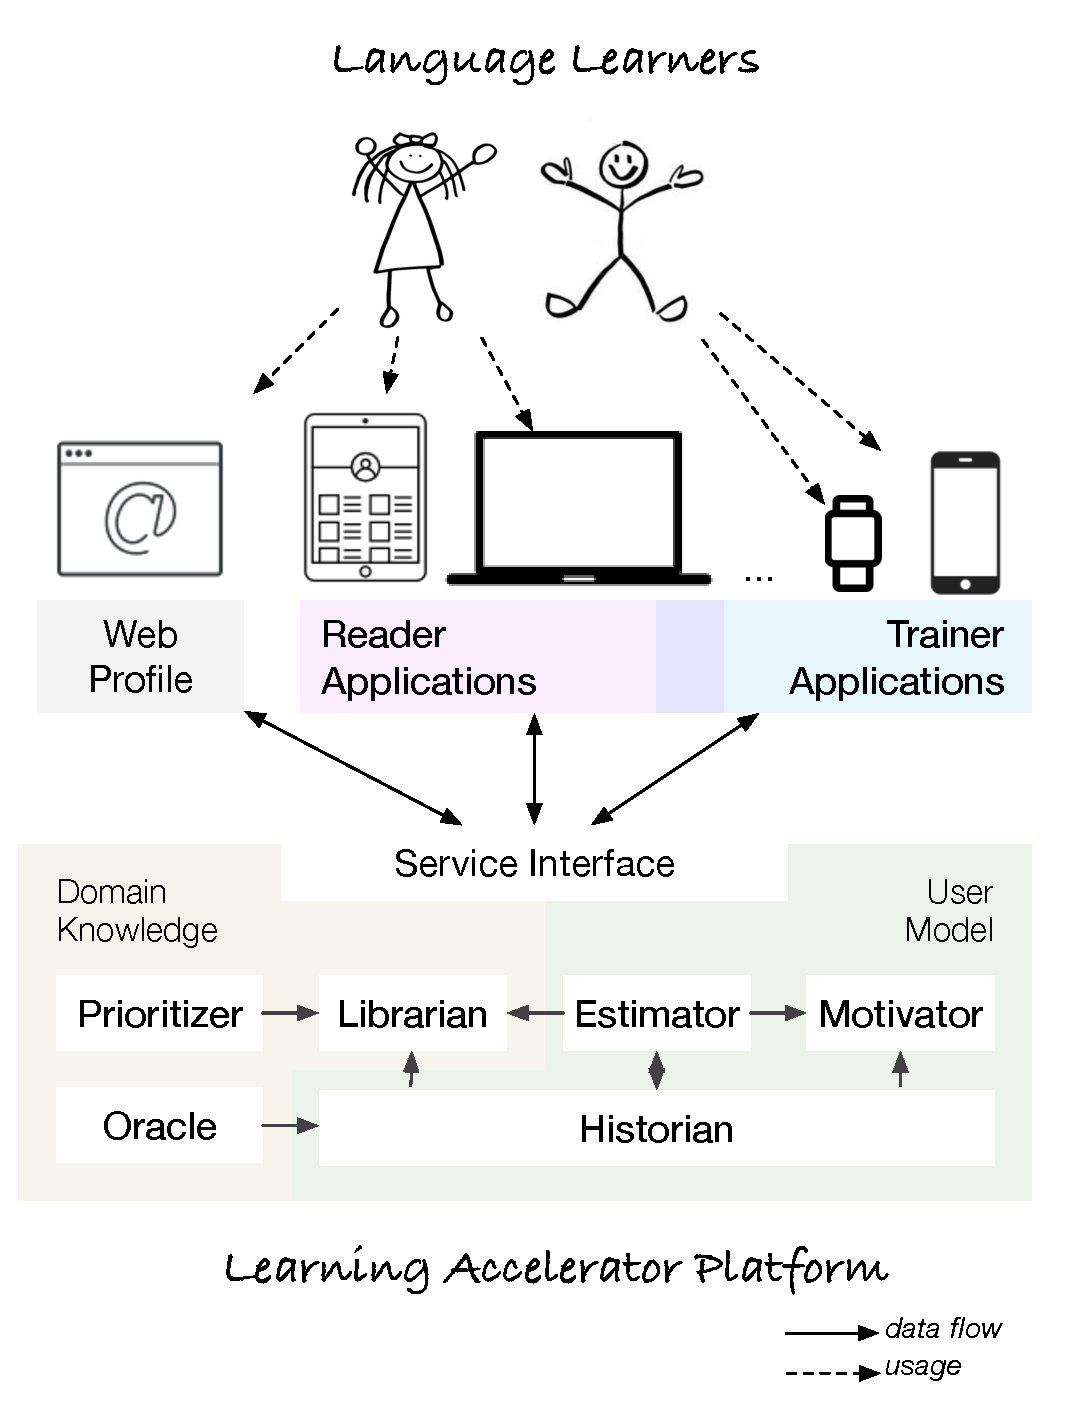
\includegraphics[width=0.96\linewidth]{images/zeeguu-architecture.pdf}
	\caption{A very high-level view of the architecture of the Zeeguu ecosystem}
	\label{fig:architecture}
\end{figure}

The figure presents explicitly only one category of actors -- the {\em language learners}. A second type of actor in the ecosystem are the {\em applicatoin developers} who build the applications with which the learners interact. There are two types of such applications: 

\begin{description}
	
	\item {\bf Reader Applications} ease the reading of materials in foreign languages. The reader applications must have at least two properties in common: 
		1) the usability of obtaining translations for unknown words in foreign language texts should be high (this is a quality attribute); 
		2) they should report back to the platform information that could be used to infer the current user knowledge (this is a functional requirement).\footnote{e.g., the words that are being looked up, the context of these words, the time spent reading an article, etc.} 

		% In particular, every word that is being translated by the user indicates his lack of knowledge with respect to that particular word, and every word that is not being translated by the user indicates their potential knowledge of that word. The context in which a word has been encountered is also useful. 
	
		\item {\bf Trainer Applications} provide exercises to accelerate the retention of individual words. Trainer applications have in common two functional properties: (1) they must request from the platform information on which words are prioritary to be studied and (2) they must provide back to the platform information about how well the learner behaved with respect to a given word\footnote{e.g., the correctness of an answer, the time to answer, etc.}.

\end{description}

Note that as the Figure \ref{fig:architecture} subtly suggests by overlapping the two corresponding blocks, the Reader and the Trainer applications need not necessarily be disjoint applications; instead one application could provide both functionalities.


The Zeeguu Platform is the core component of the learning ecosystem since it stores and orchestrates the exchange of information about the current and historical knowledge of the user. It has six main components: 

\newcommand {\archiblock}[1]{\item {\bf #1}}
\begin{enumerate}
	
		\archiblock{The Historian} is a data warehouse that sits at the core of a monitoring ecosystem. It records all the interactions of a user with knowledge based on the reports of Reader and Trainer applications.
		It uses either relational or noSql components based on the type of data.

		\archiblock{The Translator} is a service that provides translations between many pairs of languages to reader applications. It notifies the historian of every request it receives. 
		It uses adaptive strategies to choose between different backends that have different properties in terms of cost and quality.

		% all the interactions of a learner with texts in the foreign language that are mediated by the Reader applications.		%
		\archiblock{The Prioritizer} is a data mining focused component which aims at {\em ranking the information in the domain} based on a global view of its relative importance. It can be built based on statistical analysis of the learning patterns of the various leaners or based on a generic study of corpora in the target language.

		\archiblock{The Oracle} is a machine learning based agent that {\em estimates the current knowledge of the learner} based on user-specific information received from the Historian and language-specific information received from the Prioritizer. It decides what are the most likely items that must be studied by the learner. 

% TODO: Re-read since this is completely refactored
		\archiblock {The Librarian} {\em provides recommendations to the learners} about which materials are at the appropriate difficulty level but also interesting for the learner based on their personal preferences. It is implemented as a web crawler that uses natural language processing techniques but personalizes its results based on  information from the Oracle.

		% TODO: reference on gamificatoin? 
		\archiblock {The Motivator} is an agent that uses gamification techniques to keep the learner motivated. It uses information from the Historian to be able to report on a learners {\em engagement}. It uses information from the Oracle to be able to provide feedback on the actual {\em vocabulary acquisition } progress. 

\end{enumerate}



% Somewhere, we still have to discuss the question of: 
% - How are we going to maintain this ecosystem? who will provide the data storage and translation facilities for the long run? 
% - What are the incentives for new players to join the ecosystem?
% - ... 


